\documentclass[11pt,a4paper]{article}

\usepackage{tabulary}
\usepackage{tabularx}
\usepackage{booktabs}
\usepackage{array}
\usepackage[pdftex]{graphicx}
\usepackage[round]{natbib}
%\usepackage{natbib}
%\biboptions{longnamesfirst,round,semicolon}
\usepackage{a4wide}
%\usepackage{mathptmx}
\usepackage{amssymb}
\usepackage{amsmath}
\usepackage{times}
%\usepackage[sidewaysfigure]{rotating}
\usepackage{float}
%\usepackage[latin1]{inputenc}        %f{\"u}r deutsche Texte
\usepackage[T1]{fontenc}             %f{\"u}r deutsche Texte
\usepackage{srcltx}
\graphicspath{../figures/}
%\setlength{\parindent}{0pt}
%\sloppy
\begin{document}
%\begin{frontmatter}

\begin{center}
{\Large \textbf{A detailed overview of monetary policy rules in Modelbase} }
\par\end{center}

\fontsize{11}{18pt}\selectfont
%\setlength{\parindent}{0pt}

%\section{Appendix C: }

%\maketitle

\noindent The MMB 3.1 offers nine pre-programmed monetary policy rules from \cite{Taylor1993}, \cite{GerdesmeierRoffia2004},
\cite{LevinWielandWilliams2003}, \cite{SmetsWouters2007}, \cite{ChristianoEichenbaumEvans2005}, \cite{OrphanidesWieland2008}, \cite{OrphanidesWieland2013}, \cite{CMR2014} and \cite{Coenenetal2012}, along with an option for the users to specify their own rule. Table 1 shows the equation of the nine-plus-one policy rules in MMB 3.1. %\ref{tab:PolicyRules}.

\begin{table}[H]
\caption{\textsc{MONETARY POLICY RULES IN MODELBASE}}
\vspace{.2cm}
\label{tab:PolicyRules}
\begin{tabularx}{\textwidth}{ll}
\hline
&\\
\cite{Taylor1993}                  & $i_{t}^{z} = \sum_{j=0}^3 0.375 p_{t-j}^{z} +0.50 q_{t}^{z} +\eta_{t}^{i} $  \\
&\\
\cite{GerdesmeierRoffia2004}       & $i_{t}^{z} = 0.66 i_{t-1}^{z} +\sum_{j=0}^3 0.17 p_{t-j}^{z} + 0.10 q_{t}^{z} +\eta_{t}^{i}$  \\
&\\
\cite{LevinWielandWilliams2003}    & $i_{t}^{z} = 0.76 i_{t-1}^{z} +\sum_{j=0}^3 0.15 p_{t-j}^{z} +1.18 q_{t}^{z}-0.97 q_{t-1}^{z} +\eta_{t}^{i}$ \\
&\\
\cite{SmetsWouters2007}            & $i_{t}^{z} = 0.81 i_{t-1}^{z} +0.39 p_{t}^{z} +0.97 q_{t}^{z} -0.90 q_{t-1}^{z} +\eta_{t}^{i}$  \\
&\\
\cite{ChristianoEichenbaumEvans2005} & $i_{t}^{z} = 0.8 i_{t-1}^{z} +0.3 E_{t}p_{t+1}^{z} +0.08q_{t}^{z} +\eta_{t}^{i}$ \\
&\\
\cite{OrphanidesWieland2008} & $i_{t}^{z} = 2.34 E_{t}\pi_{t+3}^{z} +0.765 E_{t}q_{t+3}^{z} +\eta_{t}^{i}$ \\
&\\
\cite{OrphanidesWieland2013} & $i_{t}^{z} = i_{t-1}^{z} +0.5 \pi_{t}^{z} +0.5(q_{t}^{z}-q_{t-4}^{z}) +\eta_{t}^{i}$ \\
 &\\
\cite{CMR2014} & $i_{t}^{z} = 0.85 i_{t-1}^{z} +0.36 p_{t}^{z} + 0.05 y_{t}^{z} - 0.05 y_{t-1}^{z} +\eta_{t}^{i}$\\
&\\
\cite{Coenenetal2012} & $i_{t}^{z} = 0.7 i_{t-1}^{z} +1.25(p_{t}^{z}+ p_{t+4}^{z})$\\
&\\
User-specified rule    &{$\!\begin{aligned} 
                         i_{t}^{z} =& {\sum}_{j=1}^{j=4}\rho_{i,j}i_{t-j}^{z} +{\sum}_{j=-4}^{j=4}\rho_{\pi,j}p_{t+j}^{z} +{\sum}_{j=-4}^{j=4}\rho_{q,j}q_{t+j}^{z}\\ 
								          &+{\sum}_{j=-4}^{j=4}\rho_{y,j}y_{t+j}^{z} +\eta_{t}^{i}
								\end{aligned}$}\\
\hline
\end{tabularx}
\end{table}
\noindent In all rules, $i_t^z $ denotes the annualized quarterly money market rate; $\pi_t^z$ refers to the year-on-year rate of inflation; $ p_t^z$ is the annualized quarter-to-quarter rate of inflation; $y_t^z $ denotes the quarterly real GDP; $ q_t^z$ refers to the quarterly output gap, defined as the deviation of actual output from the level of output that would be realized if prices were flexible; $\eta_{t}^{i} $ is the common monetary policy shock.\\

\begin{itemize}
	\item The \cite{Taylor1993} rule has drawn much attention due to its precise description of the Federal Reserve's interest rate decision. A significant amount of Taylor-type rules have been developed since the 1990s.
	\item The \cite{GerdesmeierRoffia2004} rule is an augmented Taylor rule with the interest-rate smoothing term. \cite{KuesterWieland2010} use the rule to compare four euro-area models, which are included in MMB 3.1. 
	\item The \cite{LevinWielandWilliams2003} rule allows for interest-rate smoothing and reacts to lagged output gap, in addition to current output gap and current inflation. Estimation of the rule is based on the U.S. data in \cite{OrphanidesWieland1998}. \cite{LevinWielandWilliams2003} employ the rule to compare five U.S. models, which are included in MMB 3.1.
	\item The \cite{SmetsWouters2007} rule is one of the best-known rules among medium-scale new-Keynesian models. The rule, with estimation based on Bayesian techniques, includes lagged interest rate, current inflation, as well as lagged and current output similar to the \cite{LevinWielandWilliams2003} rule.
	\item The \cite{ChristianoEichenbaumEvans2005} rule, unlike the first four rules, is forward-looking and responds to inflation forecast one period ahead. The rule is an extension of  \cite{ClaridaGaliGertler1999}.
	\item The \cite{OrphanidesWieland2008} rule is forward-looking as it includes forecasts for inflation and unemployment rate three quarters ahead. Estimation of the rule is based on the FOMC's projection on inflation and unemployment rate, considering the release time of the semiannual monetary policy report to the U.S. Congress. A rule without interest-rate smoothing (the fourth column in Table 3 in \cite{OrphanidesWieland2008}) is included in MMB 3.1. The unemployment rate in the original rule is replaced by the output gap that uses Okun's law: $-2 (u-\bar{u}) \approx (y-\bar{y})$.
	\item The \cite{OrphanidesWieland2013} rule is an outcome-based simple policy rule. Change in the policy rate responds equally to the growth rate of current inflation and output gap over the last four quarters. The rule delivers fairly robust stabilization performance across 11 euro-area models, which are included in MMB 3.1.
	\item The \cite{CMR2014} rule's estimation is based on a model featuring wage and price rigidities, as well as financial frictions \`a la \cite{BernankeGertlerGilchrist1999}.
	\item The \cite{Coenenetal2012} rule is the standardized interest rate reaction function used in Figure 1 of the paper. Coefficients were set by calibration to satisfy the requirement for dynamic stability in the seven policy models in the paper. (see \cite{Coenenetal2012}, footnote 17).   
	\item The User-specified rule allows you to set desired coefficients of variables in a generalized interest rate rule. To use this option based on, for instance, the Taylor (1993) rule, as Figure \ref{img:MenuStructure3} shows , the coefficients should be set as: $ \rho_{\pi,0} = \rho_{\pi,-1} = \rho_{\pi,-2} = \rho_{\pi,-3} = 0.375, \rho_{q,0} = 0.5 $, with the rest at zero. Note that a model might not be simulated given certain calibration. The system of a proposed monetary policy rule and other model equations may violate the Blanchard-Kahn condition such that they cannot yield a unique stationary rational expectation equilibrium. There is no a hard guideline for determinacy, but \cite{LevinWielandWilliams2003} suggest several characteristics of rules that deliver a unique equilibrium: a relatively short inflation forecast horizon, a moderate degree of responsiveness to the inflation forecast, an explicit response to the current output gap and a substantial degree of policy inertia. \\

\begin{figure}[H]
\centering
\caption{\textsc{TAYLOR (1993) RULE USING THE OPTION OF USER-SPECIFIC RULE }}
\vspace{0.2cm}
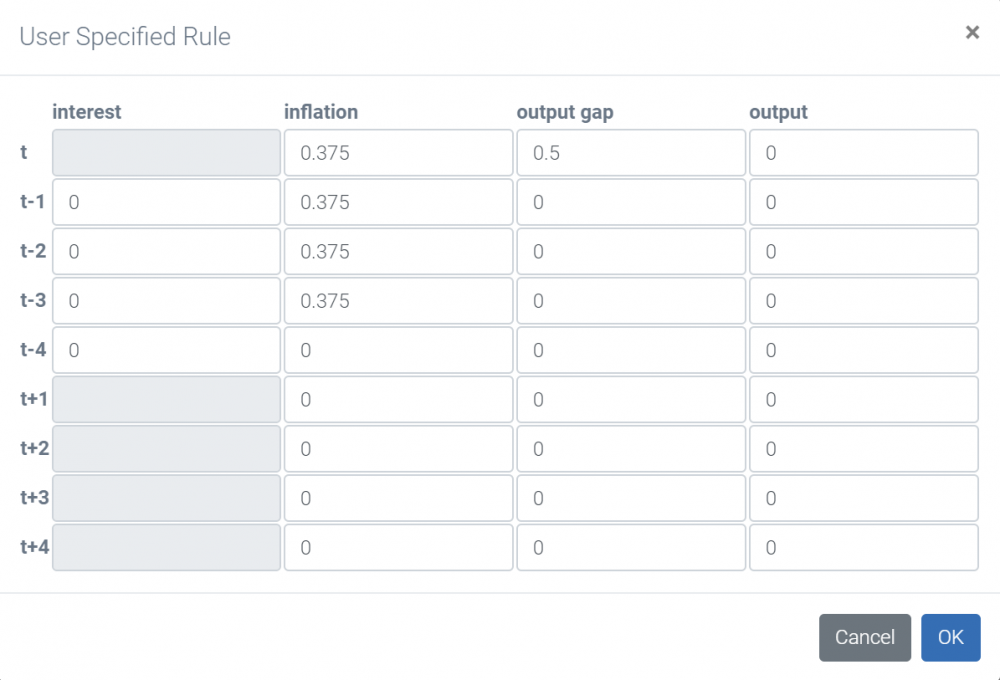
\includegraphics[width=15cm,keepaspectratio]{userrule.png}%{../figures/userrule_taylor.eps}
\label{img:MenuStructure3}
\end{figure}


\end{itemize}

\noindent The Model-specific rules are those developed exclusively for the corresponding models in each paper. They are available for the large majority of  models in MMB 3.1, with the specifications given in the respective model-specific .JSON-files in the model-specific folders listed in the directory: ....static/mmci-cli/models.

%\section*{References}
\setlength{\bibsep}{0.4\baselineskip}
\bibliographystyle{elsarticle-harv}
\bibliography{DynareModelBase}
%\nocite{*} %With this command, also those papers not cited in the text will appear in the reference list

\end{document}
